\documentclass[twoside]{book}

% Packages required by doxygen
\usepackage{fixltx2e}
\usepackage{calc}
\usepackage{doxygen}
\usepackage[export]{adjustbox} % also loads graphicx
\usepackage{graphicx}
\usepackage[utf8]{inputenc}
\usepackage{makeidx}
\usepackage{multicol}
\usepackage{multirow}
\PassOptionsToPackage{warn}{textcomp}
\usepackage{textcomp}
\usepackage[nointegrals]{wasysym}
\usepackage[table]{xcolor}

% Font selection
\usepackage[T1]{fontenc}
\usepackage[scaled=.90]{helvet}
\usepackage{courier}
\usepackage{amssymb}
\usepackage{sectsty}
\renewcommand{\familydefault}{\sfdefault}
\allsectionsfont{%
  \fontseries{bc}\selectfont%
  \color{darkgray}%
}
\renewcommand{\DoxyLabelFont}{%
  \fontseries{bc}\selectfont%
  \color{darkgray}%
}
\newcommand{\+}{\discretionary{\mbox{\scriptsize$\hookleftarrow$}}{}{}}

% Page & text layout
\usepackage{geometry}
\geometry{%
  a4paper,%
  top=2.5cm,%
  bottom=2.5cm,%
  left=2.5cm,%
  right=2.5cm%
}
\tolerance=750
\hfuzz=15pt
\hbadness=750
\setlength{\emergencystretch}{15pt}
\setlength{\parindent}{0cm}
\setlength{\parskip}{0.2cm}
\makeatletter
\renewcommand{\paragraph}{%
  \@startsection{paragraph}{4}{0ex}{-1.0ex}{1.0ex}{%
    \normalfont\normalsize\bfseries\SS@parafont%
  }%
}
\renewcommand{\subparagraph}{%
  \@startsection{subparagraph}{5}{0ex}{-1.0ex}{1.0ex}{%
    \normalfont\normalsize\bfseries\SS@subparafont%
  }%
}
\makeatother

% Headers & footers
\usepackage{fancyhdr}
\pagestyle{fancyplain}
\fancyhead[LE]{\fancyplain{}{\bfseries\thepage}}
\fancyhead[CE]{\fancyplain{}{}}
\fancyhead[RE]{\fancyplain{}{\bfseries\leftmark}}
\fancyhead[LO]{\fancyplain{}{\bfseries\rightmark}}
\fancyhead[CO]{\fancyplain{}{}}
\fancyhead[RO]{\fancyplain{}{\bfseries\thepage}}
\fancyfoot[LE]{\fancyplain{}{}}
\fancyfoot[CE]{\fancyplain{}{}}
\fancyfoot[RE]{\fancyplain{}{\bfseries\scriptsize Generated on Sun Dec 13 2015 21\+:59\+:31 for My Project by Doxygen }}
\fancyfoot[LO]{\fancyplain{}{\bfseries\scriptsize Generated on Sun Dec 13 2015 21\+:59\+:31 for My Project by Doxygen }}
\fancyfoot[CO]{\fancyplain{}{}}
\fancyfoot[RO]{\fancyplain{}{}}
\renewcommand{\footrulewidth}{0.4pt}
\renewcommand{\chaptermark}[1]{%
  \markboth{#1}{}%
}
\renewcommand{\sectionmark}[1]{%
  \markright{\thesection\ #1}%
}

% Indices & bibliography
\usepackage{natbib}
\usepackage[titles]{tocloft}
\setcounter{tocdepth}{3}
\setcounter{secnumdepth}{5}
\makeindex

% Hyperlinks (required, but should be loaded last)
\usepackage{ifpdf}
\ifpdf
  \usepackage[pdftex,pagebackref=true]{hyperref}
\else
  \usepackage[ps2pdf,pagebackref=true]{hyperref}
\fi
\hypersetup{%
  colorlinks=true,%
  linkcolor=blue,%
  citecolor=blue,%
  unicode%
}

% Custom commands
\newcommand{\clearemptydoublepage}{%
  \newpage{\pagestyle{empty}\cleardoublepage}%
}


%===== C O N T E N T S =====

\begin{document}

% Titlepage & ToC
\hypersetup{pageanchor=false,
             bookmarks=true,
             bookmarksnumbered=true,
             pdfencoding=unicode
            }
\pagenumbering{roman}
\begin{titlepage}
\vspace*{7cm}
\begin{center}%
{\Large My Project }\\
\vspace*{1cm}
{\large Generated by Doxygen 1.8.10}\\
\vspace*{0.5cm}
{\small Sun Dec 13 2015 21:59:31}\\
\end{center}
\end{titlepage}
\clearemptydoublepage
\tableofcontents
\clearemptydoublepage
\pagenumbering{arabic}
\hypersetup{pageanchor=true}

%--- Begin generated contents ---
\chapter{Hierarchical Index}
\section{Class Hierarchy}
This inheritance list is sorted roughly, but not completely, alphabetically\+:\begin{DoxyCompactList}
\item \contentsline{section}{Quiz\+Result}{\pageref{class_quiz_result}}{}
\item \contentsline{section}{Student\+Profile}{\pageref{class_student_profile}}{}
\item \contentsline{section}{User}{\pageref{class_user}}{}
\begin{DoxyCompactList}
\item \contentsline{section}{Admin\+User}{\pageref{class_admin_user}}{}
\item \contentsline{section}{Student\+User}{\pageref{class_student_user}}{}
\end{DoxyCompactList}
\end{DoxyCompactList}

\chapter{Class Index}
\section{Class List}
Here are the classes, structs, unions and interfaces with brief descriptions\+:\begin{DoxyCompactList}
\item\contentsline{section}{\hyperlink{class_admin_user}{Admin\+User} \\*\hyperlink{class_admin_user}{Admin\+User} class }{\pageref{class_admin_user}}{}
\item\contentsline{section}{\hyperlink{class_quiz_result}{Quiz\+Result} \\*\hyperlink{class_quiz_result}{Quiz\+Result} class }{\pageref{class_quiz_result}}{}
\item\contentsline{section}{\hyperlink{class_student_profile}{Student\+Profile} \\*\hyperlink{class_student_profile}{Student\+Profile} class }{\pageref{class_student_profile}}{}
\item\contentsline{section}{\hyperlink{class_student_user}{Student\+User} \\*\hyperlink{class_student_user}{Student\+User} class }{\pageref{class_student_user}}{}
\item\contentsline{section}{\hyperlink{class_user}{User} \\*Base \hyperlink{class_user}{User} class }{\pageref{class_user}}{}
\end{DoxyCompactList}

\chapter{Class Documentation}
\hypertarget{class_admin_user}{}\section{Admin\+User Class Reference}
\label{class_admin_user}\index{Admin\+User@{Admin\+User}}


\hyperlink{class_admin_user}{Admin\+User} class.  


Inheritance diagram for Admin\+User\+:\begin{figure}[H]
\begin{center}
\leavevmode
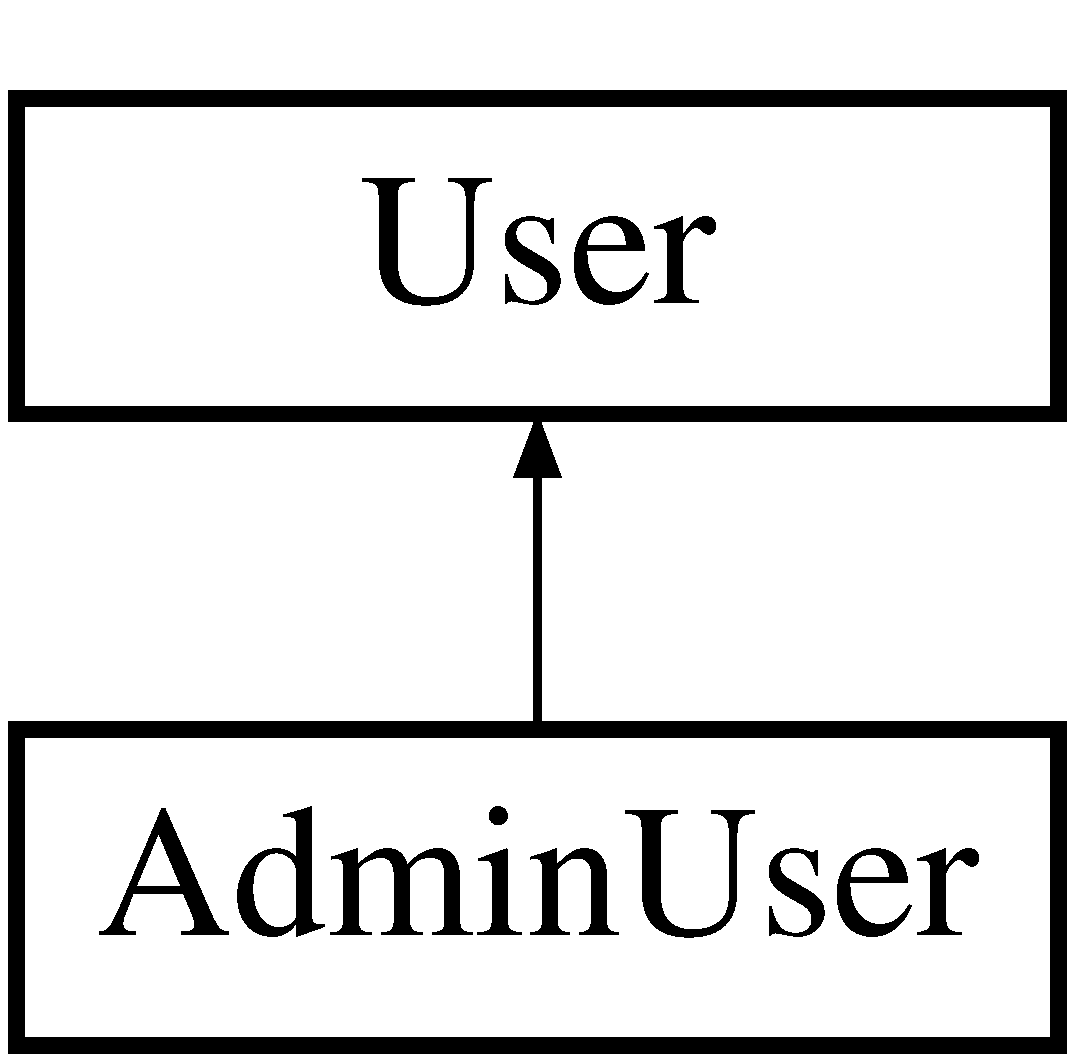
\includegraphics[height=2.000000cm]{class_admin_user}
\end{center}
\end{figure}
\subsection*{Public Member Functions}
\begin{DoxyCompactItemize}
\item 
\hyperlink{class_admin_user_a0d2bb23705126f8f07af33c915a1c21c}{Admin\+User} (string I\+D)
\begin{DoxyCompactList}\small\item\em \hyperlink{class_admin_user}{Admin\+User} constructor for admins after logging in. \end{DoxyCompactList}\item 
void \hyperlink{class_admin_user_a3f481e9aecf194dad67b6a702ed18e41}{view\+Profile} (string student\+I\+D)
\begin{DoxyCompactList}\small\item\em A member function to view the profile of a student. \end{DoxyCompactList}\end{DoxyCompactItemize}
\subsection*{Additional Inherited Members}


\subsection{Detailed Description}
\hyperlink{class_admin_user}{Admin\+User} class. 

Class for a \hyperlink{class_admin_user}{Admin\+User}, which is created by a \hyperlink{class_user}{User} logging in with admin credentials. 

\subsection{Constructor \& Destructor Documentation}
\hypertarget{class_admin_user_a0d2bb23705126f8f07af33c915a1c21c}{}\index{Admin\+User@{Admin\+User}!Admin\+User@{Admin\+User}}
\index{Admin\+User@{Admin\+User}!Admin\+User@{Admin\+User}}
\subsubsection[{Admin\+User(string I\+D)}]{\setlength{\rightskip}{0pt plus 5cm}Admin\+User\+::\+Admin\+User (
\begin{DoxyParamCaption}
\item[{string}]{I\+D}
\end{DoxyParamCaption}
)\hspace{0.3cm}{\ttfamily [inline]}}\label{class_admin_user_a0d2bb23705126f8f07af33c915a1c21c}


\hyperlink{class_admin_user}{Admin\+User} constructor for admins after logging in. 


\begin{DoxyParams}{Parameters}
{\em I\+D} & a string containing the \hyperlink{class_admin_user}{Admin\+User}\textquotesingle{}s I\+D. \\
\hline
\end{DoxyParams}


\subsection{Member Function Documentation}
\hypertarget{class_admin_user_a3f481e9aecf194dad67b6a702ed18e41}{}\index{Admin\+User@{Admin\+User}!view\+Profile@{view\+Profile}}
\index{view\+Profile@{view\+Profile}!Admin\+User@{Admin\+User}}
\subsubsection[{view\+Profile(string student\+I\+D)}]{\setlength{\rightskip}{0pt plus 5cm}void Admin\+User\+::view\+Profile (
\begin{DoxyParamCaption}
\item[{string}]{student\+I\+D}
\end{DoxyParamCaption}
)\hspace{0.3cm}{\ttfamily [inline]}}\label{class_admin_user_a3f481e9aecf194dad67b6a702ed18e41}


A member function to view the profile of a student. 


\begin{DoxyParams}{Parameters}
{\em I\+D} & a string containing the I\+D of the student whose profile is desired. \\
\hline
\end{DoxyParams}


The documentation for this class was generated from the following file\+:\begin{DoxyCompactItemize}
\item 
main.\+cpp\end{DoxyCompactItemize}

\hypertarget{class_quiz_result}{}\section{Quiz\+Result Class Reference}
\label{class_quiz_result}\index{Quiz\+Result@{Quiz\+Result}}


\hyperlink{class_quiz_result}{Quiz\+Result} class.  


\subsection*{Public Member Functions}
\begin{DoxyCompactItemize}
\item 
\hyperlink{class_quiz_result_adfc51d6f01b658543634624438bb4d1e}{Quiz\+Result} (string \hyperlink{class_quiz_result_a86aecf71051b7e6592911f0ff319d170}{date\+Of\+Quiz}, int \hyperlink{class_quiz_result_af1967ad86d0a6a544cb780a7f742c8b3}{correct\+Answers})
\begin{DoxyCompactList}\small\item\em Constructor used to generate a \hyperlink{class_quiz_result}{Quiz\+Result}. \end{DoxyCompactList}\end{DoxyCompactItemize}
\subsection*{Public Attributes}
\begin{DoxyCompactItemize}
\item 
\hypertarget{class_quiz_result_a86aecf71051b7e6592911f0ff319d170}{}string \hyperlink{class_quiz_result_a86aecf71051b7e6592911f0ff319d170}{date\+Of\+Quiz}\label{class_quiz_result_a86aecf71051b7e6592911f0ff319d170}

\begin{DoxyCompactList}\small\item\em The date the quiz was taken. \end{DoxyCompactList}\item 
\hypertarget{class_quiz_result_af1967ad86d0a6a544cb780a7f742c8b3}{}int \hyperlink{class_quiz_result_af1967ad86d0a6a544cb780a7f742c8b3}{correct\+Answers}\label{class_quiz_result_af1967ad86d0a6a544cb780a7f742c8b3}

\begin{DoxyCompactList}\small\item\em Number of correct answers during the quiz. \end{DoxyCompactList}\end{DoxyCompactItemize}


\subsection{Detailed Description}
\hyperlink{class_quiz_result}{Quiz\+Result} class. 

Class for a \hyperlink{class_quiz_result}{Quiz\+Result}. Is generated by a Quiz\+Attempt, and saved to a \hyperlink{class_student_profile}{Student\+Profile}. 

\subsection{Constructor \& Destructor Documentation}
\hypertarget{class_quiz_result_adfc51d6f01b658543634624438bb4d1e}{}\index{Quiz\+Result@{Quiz\+Result}!Quiz\+Result@{Quiz\+Result}}
\index{Quiz\+Result@{Quiz\+Result}!Quiz\+Result@{Quiz\+Result}}
\subsubsection[{Quiz\+Result(string date\+Of\+Quiz, int correct\+Answers)}]{\setlength{\rightskip}{0pt plus 5cm}Quiz\+Result\+::\+Quiz\+Result (
\begin{DoxyParamCaption}
\item[{string}]{date\+Of\+Quiz, }
\item[{int}]{correct\+Answers}
\end{DoxyParamCaption}
)\hspace{0.3cm}{\ttfamily [inline]}}\label{class_quiz_result_adfc51d6f01b658543634624438bb4d1e}


Constructor used to generate a \hyperlink{class_quiz_result}{Quiz\+Result}. 


\begin{DoxyParams}{Parameters}
{\em date\+Of\+Quiz} & the date the quiz was taken. \\
\hline
{\em answers} & Number of correct answers during the quiz. \\
\hline
\end{DoxyParams}


The documentation for this class was generated from the following file\+:\begin{DoxyCompactItemize}
\item 
main.\+cpp\end{DoxyCompactItemize}

\hypertarget{class_student_profile}{}\section{Student\+Profile Class Reference}
\label{class_student_profile}\index{Student\+Profile@{Student\+Profile}}


\hyperlink{class_student_profile}{Student\+Profile} class.  




{\ttfamily \#include $<$user.\+h$>$}

\subsection*{Public Member Functions}
\begin{DoxyCompactItemize}
\item 
\hyperlink{class_student_profile_adff542cb5595ba22e7d0f43475610ef3}{Student\+Profile} (string I\+D)
\begin{DoxyCompactList}\small\item\em \hyperlink{class_student_profile}{Student\+Profile} constructor for initialisation. \end{DoxyCompactList}\item 
void \hyperlink{class_student_profile_a52410e28b23a48921163e62689212d0c}{add\+Result} (string date\+Of\+Quiz, int correct\+Answers)
\begin{DoxyCompactList}\small\item\em A member function to add a \hyperlink{class_quiz_result}{Quiz\+Result} from a quiz attempt. \end{DoxyCompactList}\item 
void \hyperlink{class_student_profile_af2d8e1bbc6f054544607ec7d264c88a4}{print\+To\+Screen} ()
\begin{DoxyCompactList}\small\item\em A member function to print a profile to the screen. \end{DoxyCompactList}\item 
void \hyperlink{class_student_profile_a53043210f40c1b2dea4a0c43eb9dcd58}{print\+To\+File} (ostream \&output)
\begin{DoxyCompactList}\small\item\em A member function to print a profile to a specified file. \end{DoxyCompactList}\end{DoxyCompactItemize}
\subsection*{Protected Attributes}
\begin{DoxyCompactItemize}
\item 
\hypertarget{class_student_profile_a064b84fa7af49381f0e92ed0269079ce}{}string \hyperlink{class_student_profile_a064b84fa7af49381f0e92ed0269079ce}{student\+I\+D}\label{class_student_profile_a064b84fa7af49381f0e92ed0269079ce}

\begin{DoxyCompactList}\small\item\em I\+D of \hyperlink{class_student_user}{Student\+User} which owns the profile. \end{DoxyCompactList}\item 
\hypertarget{class_student_profile_a291e232fb2269319d2e3d903c8e5b5b2}{}string \hyperlink{class_student_profile_a291e232fb2269319d2e3d903c8e5b5b2}{profile\+File\+Name}\label{class_student_profile_a291e232fb2269319d2e3d903c8e5b5b2}

\begin{DoxyCompactList}\small\item\em Name of file which stores the profile. \end{DoxyCompactList}\end{DoxyCompactItemize}


\subsection{Detailed Description}
\hyperlink{class_student_profile}{Student\+Profile} class. 

Class for a \hyperlink{class_student_profile}{Student\+Profile}, which is a log of all quiz results for a particular student. 

\subsection{Constructor \& Destructor Documentation}
\hypertarget{class_student_profile_adff542cb5595ba22e7d0f43475610ef3}{}\index{Student\+Profile@{Student\+Profile}!Student\+Profile@{Student\+Profile}}
\index{Student\+Profile@{Student\+Profile}!Student\+Profile@{Student\+Profile}}
\subsubsection[{Student\+Profile(string I\+D)}]{\setlength{\rightskip}{0pt plus 5cm}Student\+Profile\+::\+Student\+Profile (
\begin{DoxyParamCaption}
\item[{string}]{I\+D}
\end{DoxyParamCaption}
)\hspace{0.3cm}{\ttfamily [inline]}}\label{class_student_profile_adff542cb5595ba22e7d0f43475610ef3}


\hyperlink{class_student_profile}{Student\+Profile} constructor for initialisation. 


\begin{DoxyParams}{Parameters}
{\em I\+D} & a string containing the \hyperlink{class_student_user}{Student\+User}\textquotesingle{}s I\+D. \\
\hline
\end{DoxyParams}


\subsection{Member Function Documentation}
\hypertarget{class_student_profile_a52410e28b23a48921163e62689212d0c}{}\index{Student\+Profile@{Student\+Profile}!add\+Result@{add\+Result}}
\index{add\+Result@{add\+Result}!Student\+Profile@{Student\+Profile}}
\subsubsection[{add\+Result(string date\+Of\+Quiz, int correct\+Answers)}]{\setlength{\rightskip}{0pt plus 5cm}void Student\+Profile\+::add\+Result (
\begin{DoxyParamCaption}
\item[{string}]{date\+Of\+Quiz, }
\item[{int}]{correct\+Answers}
\end{DoxyParamCaption}
)\hspace{0.3cm}{\ttfamily [inline]}}\label{class_student_profile_a52410e28b23a48921163e62689212d0c}


A member function to add a \hyperlink{class_quiz_result}{Quiz\+Result} from a quiz attempt. 


\begin{DoxyParams}{Parameters}
{\em date\+Of\+Quiz} & the date the quiz was taken. \\
\hline
{\em correct\+Answers} & the number of questions answered correctly. \\
\hline
\end{DoxyParams}
\hypertarget{class_student_profile_a53043210f40c1b2dea4a0c43eb9dcd58}{}\index{Student\+Profile@{Student\+Profile}!print\+To\+File@{print\+To\+File}}
\index{print\+To\+File@{print\+To\+File}!Student\+Profile@{Student\+Profile}}
\subsubsection[{print\+To\+File(ostream \&output)}]{\setlength{\rightskip}{0pt plus 5cm}void Student\+Profile\+::print\+To\+File (
\begin{DoxyParamCaption}
\item[{ostream \&}]{output}
\end{DoxyParamCaption}
)\hspace{0.3cm}{\ttfamily [inline]}}\label{class_student_profile_a53043210f40c1b2dea4a0c43eb9dcd58}


A member function to print a profile to a specified file. 


\begin{DoxyParams}{Parameters}
{\em \&output} & a pointer to the output file stream to print to. \\
\hline
\end{DoxyParams}
\hypertarget{class_student_profile_af2d8e1bbc6f054544607ec7d264c88a4}{}\index{Student\+Profile@{Student\+Profile}!print\+To\+Screen@{print\+To\+Screen}}
\index{print\+To\+Screen@{print\+To\+Screen}!Student\+Profile@{Student\+Profile}}
\subsubsection[{print\+To\+Screen()}]{\setlength{\rightskip}{0pt plus 5cm}void Student\+Profile\+::print\+To\+Screen (
\begin{DoxyParamCaption}
{}
\end{DoxyParamCaption}
)\hspace{0.3cm}{\ttfamily [inline]}}\label{class_student_profile_af2d8e1bbc6f054544607ec7d264c88a4}


A member function to print a profile to the screen. 

Just calls print\+To\+File, but passes it the console output instead of a file. 

The documentation for this class was generated from the following file\+:\begin{DoxyCompactItemize}
\item 
user.\+h\end{DoxyCompactItemize}

\hypertarget{class_student_user}{}\section{Student\+User Class Reference}
\label{class_student_user}\index{Student\+User@{Student\+User}}


\hyperlink{class_student_user}{Student\+User} class.  


Inheritance diagram for Student\+User\+:\begin{figure}[H]
\begin{center}
\leavevmode
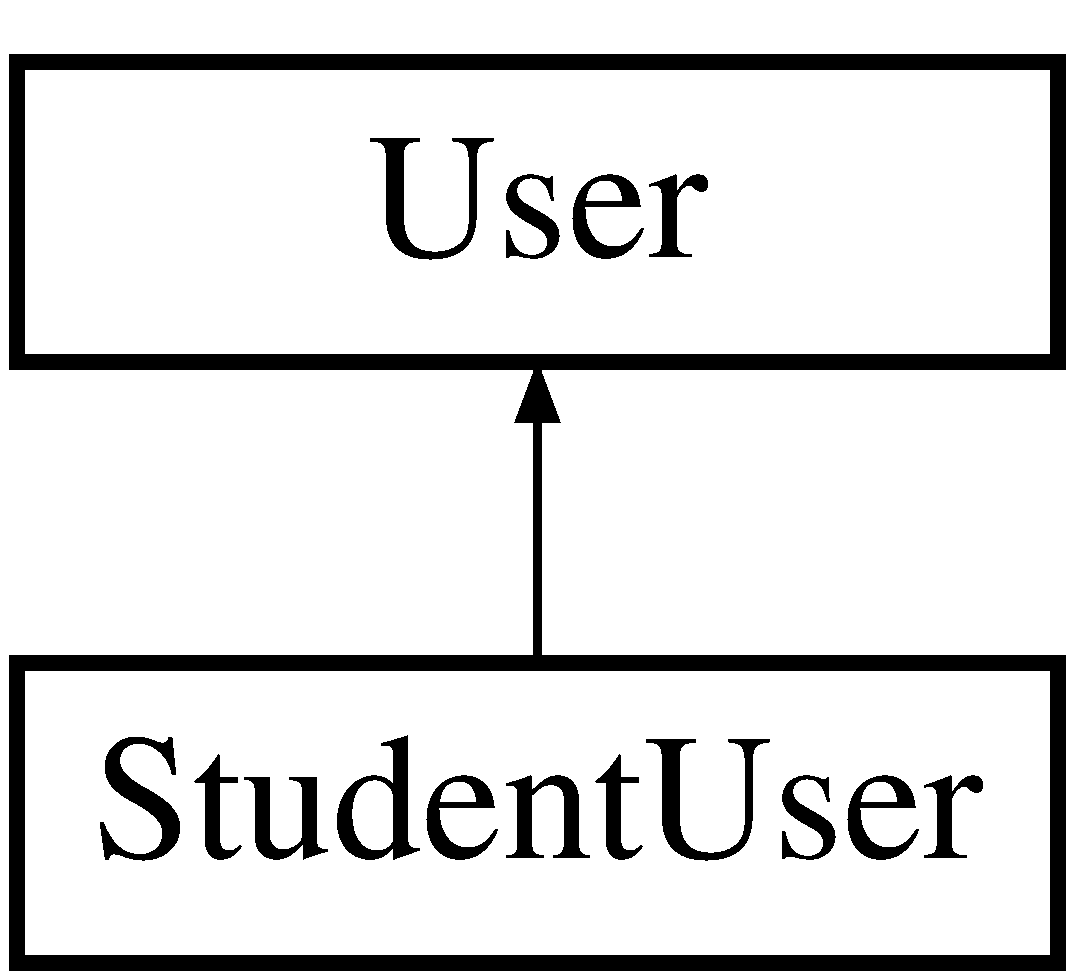
\includegraphics[height=2.000000cm]{class_student_user}
\end{center}
\end{figure}
\subsection*{Public Member Functions}
\begin{DoxyCompactItemize}
\item 
\hyperlink{class_student_user_ad518425f2cf0507128d638be6bb869d0}{Student\+User} (string I\+D)
\begin{DoxyCompactList}\small\item\em \hyperlink{class_student_user}{Student\+User} constructor for students after logging in. \end{DoxyCompactList}\item 
\hypertarget{class_student_user_a07d679b3034bf8c2d70dcda7b196fd6b}{}void \hyperlink{class_student_user_a07d679b3034bf8c2d70dcda7b196fd6b}{take\+Quiz} ()\label{class_student_user_a07d679b3034bf8c2d70dcda7b196fd6b}

\begin{DoxyCompactList}\small\item\em A member function to attempt a quiz. \end{DoxyCompactList}\end{DoxyCompactItemize}
\subsection*{Protected Member Functions}
\begin{DoxyCompactItemize}
\item 
\hypertarget{class_student_user_ace0179d78b516453d662b89d21438888}{}\hyperlink{class_student_profile}{Student\+Profile} \hyperlink{class_student_user_ace0179d78b516453d662b89d21438888}{profile} ()\label{class_student_user_ace0179d78b516453d662b89d21438888}

\begin{DoxyCompactList}\small\item\em Student\textquotesingle{}s profile containing previous quiz results. \end{DoxyCompactList}\end{DoxyCompactItemize}
\subsection*{Additional Inherited Members}


\subsection{Detailed Description}
\hyperlink{class_student_user}{Student\+User} class. 

Class for a \hyperlink{class_student_user}{Student\+User}, which is created by a \hyperlink{class_user}{User} logging in with student credentials. 

\subsection{Constructor \& Destructor Documentation}
\hypertarget{class_student_user_ad518425f2cf0507128d638be6bb869d0}{}\index{Student\+User@{Student\+User}!Student\+User@{Student\+User}}
\index{Student\+User@{Student\+User}!Student\+User@{Student\+User}}
\subsubsection[{Student\+User(string I\+D)}]{\setlength{\rightskip}{0pt plus 5cm}Student\+User\+::\+Student\+User (
\begin{DoxyParamCaption}
\item[{string}]{I\+D}
\end{DoxyParamCaption}
)\hspace{0.3cm}{\ttfamily [inline]}}\label{class_student_user_ad518425f2cf0507128d638be6bb869d0}


\hyperlink{class_student_user}{Student\+User} constructor for students after logging in. 


\begin{DoxyParams}{Parameters}
{\em I\+D} & a string containing the \hyperlink{class_student_user}{Student\+User}\textquotesingle{}s I\+D. \\
\hline
\end{DoxyParams}


The documentation for this class was generated from the following file\+:\begin{DoxyCompactItemize}
\item 
main.\+cpp\end{DoxyCompactItemize}

\hypertarget{class_user}{}\section{User Class Reference}
\label{class_user}\index{User@{User}}


Base \hyperlink{class_user}{User} class.  




{\ttfamily \#include $<$user.\+h$>$}

Inheritance diagram for User\+:\begin{figure}[H]
\begin{center}
\leavevmode
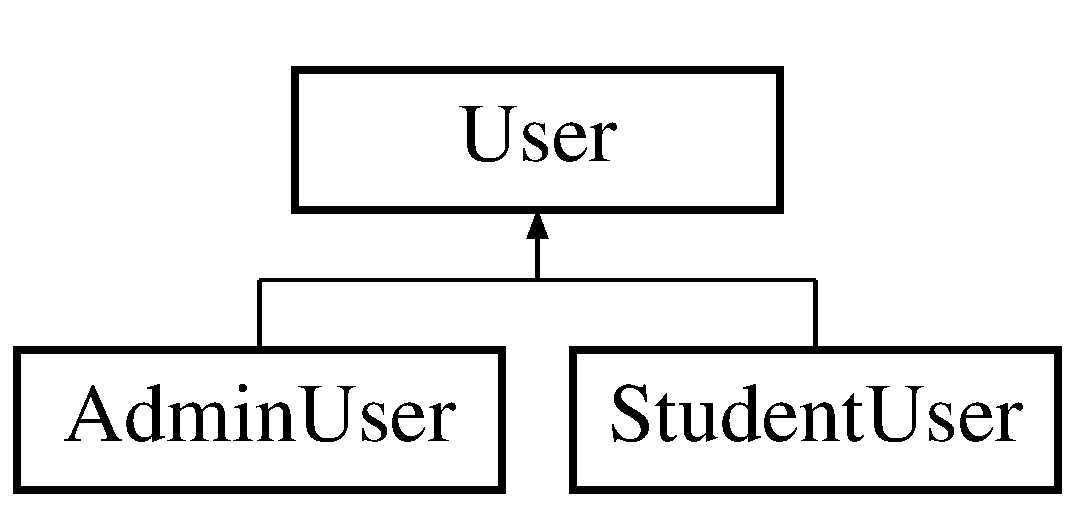
\includegraphics[height=2.000000cm]{class_user}
\end{center}
\end{figure}
\subsection*{Public Member Functions}
\begin{DoxyCompactItemize}
\item 
\hyperlink{class_user_a474a84c2e37b139228018a1aa9e814f7}{User} (string I\+D)
\begin{DoxyCompactList}\small\item\em A constructor for creating a new \hyperlink{class_user}{User} with the provided user\+I\+D. \end{DoxyCompactList}\end{DoxyCompactItemize}
\subsection*{Protected Attributes}
\begin{DoxyCompactItemize}
\item 
\hypertarget{class_user_a22f9e8d9729d3595e4ea9af8faea8abc}{}string \hyperlink{class_user_a22f9e8d9729d3595e4ea9af8faea8abc}{user\+I\+D}\label{class_user_a22f9e8d9729d3595e4ea9af8faea8abc}

\begin{DoxyCompactList}\small\item\em \hyperlink{class_user}{User} I\+D variable. \end{DoxyCompactList}\item 
\hypertarget{class_user_a6ae9d72fbd1c50a602b284b5fc659be7}{}char \hyperlink{class_user_a6ae9d72fbd1c50a602b284b5fc659be7}{permission\+Level}\label{class_user_a6ae9d72fbd1c50a602b284b5fc659be7}

\begin{DoxyCompactList}\small\item\em \hyperlink{class_user}{User} permission level (higher = more permissions). \end{DoxyCompactList}\end{DoxyCompactItemize}


\subsection{Detailed Description}
Base \hyperlink{class_user}{User} class. 

Abstract base class \hyperlink{class_user}{User}, to be used to implement different types of users. 

\subsection{Constructor \& Destructor Documentation}
\hypertarget{class_user_a474a84c2e37b139228018a1aa9e814f7}{}\index{User@{User}!User@{User}}
\index{User@{User}!User@{User}}
\subsubsection[{User(string I\+D)}]{\setlength{\rightskip}{0pt plus 5cm}User\+::\+User (
\begin{DoxyParamCaption}
\item[{string}]{I\+D}
\end{DoxyParamCaption}
)\hspace{0.3cm}{\ttfamily [inline]}}\label{class_user_a474a84c2e37b139228018a1aa9e814f7}


A constructor for creating a new \hyperlink{class_user}{User} with the provided user\+I\+D. 


\begin{DoxyParams}{Parameters}
{\em I\+D} & a string containing the \hyperlink{class_user}{User}\textquotesingle{}s I\+D. \\
\hline
\end{DoxyParams}


The documentation for this class was generated from the following file\+:\begin{DoxyCompactItemize}
\item 
user.\+h\end{DoxyCompactItemize}

%--- End generated contents ---

% Index
\backmatter
\newpage
\phantomsection
\clearemptydoublepage
\addcontentsline{toc}{chapter}{Index}
\printindex

\end{document}
